\chapter{Results} \label{chap_4}
\ \\

All collected bugs were appropriately deduplicated according to the methodology described in \ref{bug_dedup}: to do this, I used several Python scripts (one for each sanitizer and one for Valgrind) that analyzed the logs generated during each fuzzing session, and deduplication was performed using as reference the error type and the last 3 stack entries from where the error occurred.

Then, \textit{bug triage} was performed, analyzing more in-depth where the bug occurred, why it happened and assigning a priority in the range "Low", "Medium" and "High". This required a manual investigation of each bug individually, statically and dynamically (when available), to have a more clear understanding of the problem and potentially provide suggestions to the developers regarding the fix.
This step was also important to refine the previous deduplication step, as two inputs that triggered (apparently) different bugs may only have distinct stack flows: if the bug originated from the same function, it meant that two different execution flows triggered the same error. In this case, a common practice is to fix one of them and then use the other input as an additional check for correctness.

Finally, all recorded bugs for a project, along with their log and fuzz targets, were reported to their respective developers according to their preferred communication method: almost all reports were sent using GitHub's integrated issue tracker, some required a subscription to a proprietary issue tracking platform, and a few of them were sent via emails.
\newline

At the moment of writing, unfortunately, not all developers answered and/or acknowledged the reported bugs.



\newpage
\section{OSS-Fuzz}
\begin{table}[h!]
\small
\makebox[0.95\textwidth]{\begin{tabular}{|l|l|l|l|l|l|l|l|l|}
\hline
\textbf{Project} & \textbf{Sanitizers} & \textbf{Queue size} & \textbf{Crashes} & \textbf{ASan} & \textbf{Valgrind} & \textbf{UBSan} & \textbf{Total} & \textbf{Confirmed}  \\ 
\hline
binutils         & ALL                 & $20,274$            & $0$              & $0$           & $1$           & $0$            & $1$             & $1$                 \\
harfbuzz         & ALL                 & $23,357$            & $0$              & $0$           & $1$           & $0$            & $1$             & $1$                 \\
imagemagick      & ALL                 & $9,470$             & $0$              & $0$           & $6$           & $1$            & $7$             & $1$                 \\
libxml2          & ALL                 & $13,474$            & $0$              & $0$           & $0$           & $0$            & $0$             & $0$                 \\
skia             & ALL                 & $18,295$            & $0$              & $0$           & $0$           & $0$            & $0$             & $0$                 \\ 
\hline
gpsd             & A+M       & $5404$  & $0$                 & $0$              & $0$           & $0$           & $0$             & $0$                 \\
libyang          & A+M                 & $8,745$             & $0$              & $0$           & $0$           & $0$            & $0$             & $0$                 \\
llvm             & A+M                 & $10,657$             & $0$              & $21$           & $7$           & $0$            & $28$             & $17$                 \\
openjpeg         & A+M                 & $8,856$             & $0$              & $0$           & $0$           & $1$            & $1$             & $0$                 \\
wasmedge         & A+M                 & $9,454$             & $0$              & $0$           & $0$           & $0$            & $0$             & $0$                 \\
\hline
cairo            & A+UB                & $15,870$            & $0$              & $1$           & $1$           & $28$           & $30$            & $0$                 \\
clamav           & A+UB                & $6,742$             & $0$              & $0$           & $0$           & $2$            & $2$             & $0$                 \\
freerdp          & A+UB                & $7,607$             & $0$              & $0$           & $0$           & $1$            & $1$             & $1$                 \\
tarantool        & A+UB                & $10,987$            & $0$              & $0$           & $1$           & $0$            & $1$             & $1$                 \\
vlc              & A+UB                & $16,018$            & $2$              & $1$           & $2$           & $4$            & $9$             & $5$                 \\ 
\hline
fwupd            & ASan only                & $5,843$             & $0$              & $0$           & $0$           & $0$            & $0$             & $0$                 \\
glslang          & ASan only                & $14,534$            & $0$              & $1$           & $1$           & $0$            & $1$             & $1$                 \\
inchi            & ASan only                & $12,034$            & $0$              & $1$           & $4$           & $3$            & $8$             & $8$                 \\
radare2          & ASan only                & $9,914$             & $0$              & $1$           & $0$           & $9$            & $10$            & $10$                \\
zeek             & ASan only                & $8,390$             & $0$              & $0$           & $1$           & $5$            & $6$             & $6$                 \\ 
\hline
fluent-bit       & NONE                & $4,968$             & $0$              & $0$           & $1$           & $1$            & $2$             & $2$                 \\
gpac             & NONE                & $22,917$            & $2$         & $0$           & $25$          & $0$            & $27$            & $27$                \\
libdwarf         & NONE                & $7,667$             & $0$              & $0$           & $0$           & $0$            & $0$             & $0$                 \\
libredwg         & NONE                & $46,160$            & $0$              & $1$           & $3$           & $0$            & $4$             & $4$                 \\
serenity         & NONE                & $9,940$             & $0$              & $0$           & $1$           & $1$            & $2$             & $2$                 \\
\hline
TOTAL BUGS   &   &   &$4$   &$27$   &$55$   &$56$   &$141$   &$87$       \\
\hline
\end{tabular}}
\vspace{10pt}
\caption{Bugs collected by OSS-Fuzz projects}
\label{ossfuzz-table}
\end{table}
Table \ref{ossfuzz-table} shows the aggregated results for OSS-Fuzz, dividing bugs per category and showing the total number of bugs found compared to the number of bugs that were confirmed by the respective developers after being reported. While it is important to note that this is a very small subset of projects tested (25 out of 1000+) and is not representative of the entire OSS-Fuzz campaign, it is still a good indicator that there are indeed bugs that these frameworks are missing.

This analysis found a total of 141 bugs (an average of 5.64 bugs per project). In total, 35 bugs out of 141 were found by enabling new sanitizers for the first time in a project: this result is expected since that software was never tested for that class of bugs and doing it for the first time will surely detect new bugs. On the other hand, the remaining 100 bugs were found using sanitizers that were already enabled in the target software: this result is more interesting, because it means that even if a sanitizer is enabled, OSS-Fuzz may detect a bug but fails to report it.

The analysis of the \textit{llvm} project yielded a total of 28 bugs, mostly stack exhaustion bugs which cannot reproduce outside of builds with ASan enabled. This is a known issue with ASan as it increases the size of stack objects thus exhausting the stack faster than the program would without the sanitizer: we further confirmed that, by doubling the maximum size of the stack, even the ASan build could not exhaust the stack. We still reported these issues and deferred to the developers the choice on whether these issues are relevant, and the discussion is still ongoing.

We can also infer the popularity of each sanitizer. ASan is the most widely used, which is reflected by the number of bugs it found. UBSan is also among the most used ones, although the statistic shown here is biased by "Cairo": while this project is affected by many UB bugs, specifically the improper conversion of data between different types, almost all previous reports on the issue tracker related to similar problems were simply marked as "WontFix". Finally, almost all projects had (at least) 1 memory bug discovered using Valgrind, which shows how MSan is often discarded due to its reports having too many false positives when the program is not properly compiled with this sanitizer. 



\newpage
\subsection{Case study: GPAC}
The \textit{"GPAC Project on Advanced Content"} (abbreviated \textit{GPAC}) \cite{gpac} is a free and open-source multimedia framework that provides tools to process, inspect, package, stream, media playback and interact with media content, making it a popular choice also among major broadcasters such as Netflix.

Its analysis yielded a total of 27 bugs, 2 crashes and 25 memory-related bugs.
The crashes were related to a SEGV signal sent as a consequence of the process attempting to access address \verb|0x0| (i.e. zero page), which is the first page of a computer's memory and whose access is prohibited and causes an access violation fault, shown below:
\begin{figure}[h]
\makebox[\textwidth][c]{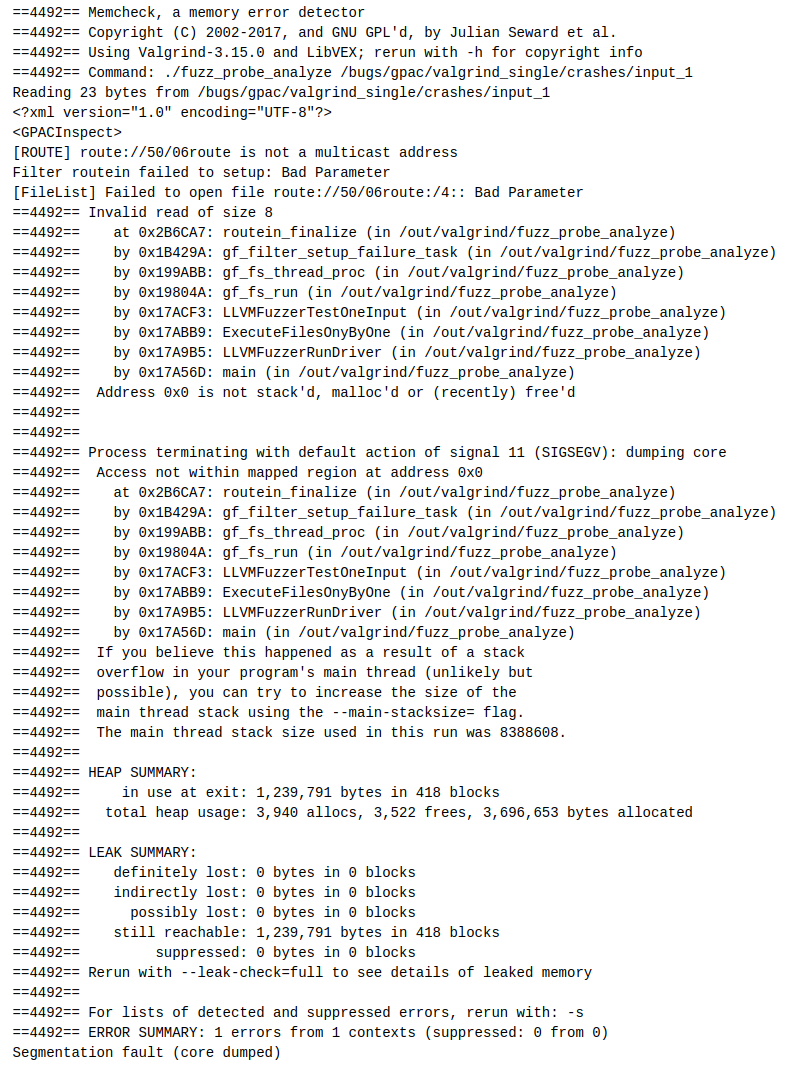
\includegraphics[width=0.55\paperwidth]{foto/segv_gpac.png}}
\caption{Memory access violation reported by Valgrind}
\label{fig:segv_gpac}
\end{figure}
\ \\

It is interesting to note that these bugs have already been reported by ClusterFuzz when discovered by this work and, more importantly, they were still in the bug disclosure windows: this meant that the inputs causing these bugs were not meant to be added to later fuzzing queues and should have not been publicly accessible and available, due to obvious security implications.

The remaining 25 memory bugs were all related to use-of-uninitialized-memory (UUM) and memory-bound errors. More specifically, they can be divided into three categories according to Valgrind:
\begin{itemize}
    \item \textit{conditional jump or move depends on uninitialized value}: happens when an \verb|if| statement is based on a variable whose value is uninitialized
    \item \textit{use of uninitialized value in function [...]}: happens when one (or more) of the parameters passed to an invoked function are uninitialized
    \item \textit{invalid read of size [...]}: happens when a read/write operation performed overruns the provided buffer, as the content outside of a buffer could be anything
\end{itemize}

After reporting the UUM bugs and having the pleasure of interacting with the CEO of GPAC itself, we were happy to discover all bugs fixed in just a few days. The developers created a public commit \cite{gpac_commit} to explain the issues discovered and reassure everyone that they did not pose a security concern, as they believe the path to exploitation is difficult. However, they agreed on the fact that such bugs could be resolved by trivial and obvious corrections, and the existence of such issues shows that they need to be more vigilant: specifically, most of the problems mentioned originated from local structures declared but left uninitialized, and buffer-related operations with no checks regarding the size of the data passed to the buffer as well as recalling that most read/write functions return the number of bytes actually read/written.
They concluded by expressing their gratitude, as they have recently been battling with seemingly random bugs causing disruptions with the normal functionality of the program, therefore the report has been valuable in helping them to remove uninitialized variables that were leading to undefined behavior.

This project was a clear example of the importance of using sanitizers during tests, as they highlighted simple and trivial errors that would otherwise be easily overlooked during a manual analysis of the code, but still that greatly helped them in improving the user experience by removing unwanted behavior.








\newpage
\subsection{Case study: VLC}
The \textit{VLC Media Player} (commonly known as \textit{VLC}) \cite{vlc} is a free and open-source media player software and streaming media server developed by the "VideoLAN Project", supporting many audio and video compression methods, file formats and providing many free decoding and encoding libraries.

Its analysis yielded a total of 9 bugs spread across all categories: 2 crashes, 1 heap-buffer overflow, 2 memory-related bugs and 4 undefined-behaviors.
The heap-buffer overflow bug was initially presented as an ASan bug related to an invocation of \verb|memcpy| that was copying a structure into another one of the same type, which initially left the developers a bit perplexed. After further analysis, they discovered that the input provided was triggering some strange behavior in another function of their program, whose output led to incorrect usage of the copy function and therefore the buffer overflow.
The crashes were both related to a SEGV signal sent as a consequence of the process attempting to access a low address that was not mapped within the process's memory region, causing an access violation fault: both problems originated from a series of read/write operations performed on uninitialized values causing undefined behavior, ultimately leading to the process accessing an erroneous address.
The first memory bug was related to a memory-bound error caused by several read operations overrunning the provided buffers, leading to undefined behavior. At the moment of writing, the problem has yet to be fixed because the developers are discussing whether to rewrite or remove the source file causing the problem, as they argue that it is very insecure and could pose a threat to the overall security of the product.
The second memory bug was related to a use-of-uninitialized-memory (UUM) bug when opening a provided input media file. At the moment of writing, a fix has been proposed but it has yet to be merged with the main code.
Finally, the undefined-behavior (UB) bugs were all related to signed integer-overflow errors, which are relatively easy to fix. Yet, at the moment of writing, they have not been acknowledged by the developers.

This project was a clear example of the most common behavior encountered during this work when interacting with open-source developers.
When presented with bugs that could potentially lead to vulnerabilities or problems in the normal functionalities of their program, their response is usually quick and the problem is fixed in a short amount of time. 
Instead, when the problems have low or negligible priority (like the undefined-behavior bugs), they either ignore the reports or acknowledge their existence and postpone them indefinitely.



\newpage
\section{FuzzBench}
\begin{table}[h]
\small
\makebox[0.96\textwidth]{\begin{tabular}{|l|l|l|l|l|l|l|l|}
\hline
\textbf{Project} & \textbf{Sanitizers} & \textbf{Queue size} & \textbf{Crashes} & \textbf{ASan} & \textbf{UBSan} & \textbf{Total} & \textbf{Confirmed}  \\ 
\hline
bloaty   &NONE   &$2349$   &$0$   &$0$   &$2$   &$2$   &$2$ \\
curl   &NONE   &$0$   &$0$   &$0$   &$0$   &$0$   &$0$ \\
freetype2   &ALL   &$0$   &$0$   &$0$   &$0$   &$0$   &$0$ \\
harfbuzz   &ALL   &$34634$   &$0$   &$0$   &$0$   &$0$   &$0$ \\
jsoncpp   &A+UB   &$0$   &$0$   &$0$   &$0$   &$0$   &$0$ \\
lcms   &ALL   &$30526$   &$0$   &$0$   &$0$   &$0$   &$0$ \\
libjpeg-turbo   &ALL   &$0$   &$0$   &$0$   &$0$   &$0$   &$0$ \\
libpcap   &ALL   &$111$   &$0$   &$0$   &$0$   &$0$   &$0$ \\
libpng   &ALL   &$0$   &$0$   &$0$   &$0$   &$0$   &$0$ \\
libxml2   &ALL   &$1961857$   &$0$   &$0$   &$0$   &$0$   &$0$ \\
mbedtls   &NONE   &$1$   &$0$   &$0$   &$0$   &$0$   &$0$ \\
openssl   &A+UB   &$0$   &$0$   &$0$   &$0$   &$0$   &$0$ \\
openthread   &A+UB   &$0$   &$0$   &$0$   &$0$   &$0$   &$0$ \\
php   &ALL   &$202235$   &$0$   &$0$   &$0$   &$0$   &$0$ \\
proj4   &NONE   &$208971$   &$0$   &$0$   &$0$   &$0$   &$0$ \\
re2   &ALL   &$0$   &$0$   &$0$   &$0$   &$0$   &$0$ \\
sqlite3   &ALL   &$0$   &$0$   &$0$   &$0$   &$0$   &$0$ \\
systemd   &ALL   &$238072$   &$0$   &$0$   &$0$   &$0$   &$0$ \\
vorbis   &A+M   &$0$   &$0$   &$0$   &$0$   &$0$   &$0$ \\
woff2   &ALL   &$0$   &$0$   &$0$   &$0$   &$0$   &$0$ \\
zlib   &ALL   &$0$   &$0$   &$0$   &$0$   &$0$   &$0$ \\
\hline
arrow   &NONE   &$1163787$   &$0$   &$0$   &$0$   &$0$   &$0$ \\
aspell   &A+UB   &$919701$   &$0$   &$0$   &$2$   &$2$   &$2$ \\
assimp   &A+UB   &$312651$   &$43$   &$104$   &$13$   &$160$   &$55$ \\
ffmpeg   &ALL   &$212617$   &$0$   &$0$   &$6$   &$6$   &$0$ \\
file   &A+UB   &$1916360$   &$0$   &$0$   &$0$   &$0$   &$0$ \\
grok   &ALL   &$1492374$   &$0$   &$2$   &$15$   &$17$   &$17$ \\
libaom   &ALL   &$19729$   &$0$   &$0$   &$0$   &$0$   &$0$ \\
\hline
TOTAL BUGS   &   &   &$43$   &$106$   &$38$   &$187$   &$74$          \\
\hline
\end{tabular}}
\vspace{10pt}
\caption{Bugs collected by Fuzzbench and SBFT'23 benchmarks}
\label{fuzzbench-table}
\end{table}
Table \ref{fuzzbench-table} shows the aggregated results for FuzzBench, dividing bugs per category and showing the total number of bugs found compared to the number of bugs that were confirmed by the respective developers after being reported. For the sake of completeness, the table also distinguishes between the standard FuzzBench benchmarks (above) and the "SBFT '23" benchmarks (below), and reports the sanitizers regularly used by the OSS-Fuzz counterpart of the selected projects.

It is immediate to see that all bugs came from the "SBFT '23" benchmarks: these results were unexpected, given that these programs have been already tested extensively during the tool competition hosted by this conference, especially "ASSIMP" which is responsible for the majority of them. These results show the importance of double-checking the possible presence of a bug found in an older version of a software in the latest version as well. The bugs we found were detected more than a year ago but left unreported until now: an attacker could have just downloaded data from the SBFT '23 tests and have access to security-relevant bugs with very low effort.



\subsection{Case study: ASSIMP}
The \textit{"Open Asset Import Library"} (abbreviated \textit{ASSIMP}) \cite{assimp} is a cross-platform library to import 3D models into a shared, in-memory immediate format, also providing a common API for different 3D asset file formats.

Its analysis yielded a total of 160 bugs, 96 of which were unreported, divided as follows: 1 stack-buffer-overflow, 1 stack-overflow, 71 heap-buffer-overflows, 20 crashes and 3 undefined behaviors. The stack-buffer-overflow error was related to a \verb|memcpy| invocation not properly checking the length of the involved buffers, eventually overriding the stack and causing a segmentation fault. The stack-overflow was triggered by an \verb|open| function triggered in a never-ending loop, eventually leading to stack exhaustion. The heap-buffer-overflows and crashes were mostly related to improper sanitizations of user inputs when performing memory accesses, eventually also leading to segmentation faults. All the aforementioned scenarios are some of the most common methodologies that malicious people use when exploiting a program to gain control of your system, therefore fixing them would be crucial.

%\matteo{The text below can be used if they don't answer by the time you have to submit your thesis (a plausible scenario). If they do, then we can change it, but at least you have a backup plan. Your old text is still commented down here}

We reported all the bugs we found with a (private) security report through the GitHub platform this project uses. At the time of writing, the developers have not yet publicly acknowledged the existence of those bugs, but they have started providing fixes to them. Given the high number of reported bugs, it is reasonable to expect the bug-fixing process to take some time, but it will eventually lead to a much safer and, hopefully, bug-free library. 


% \ziosaba{Waiting for response, add more later...}


% Given the importance of this project, as its popularity and widespread usage allowed it to enter the strict OSS-Fuzz eligibility requirements, we argue it is unacceptable to have this many unresolved bugs. \matteo{There is no need to be this harsh on them, it can be seen as unprofessional at the very least}







\newpage
\section{Developers' responses}
This study has shown that developers have different approaches to bug reporting. 

The OSS-Fuzz reports were submitted in September, and at the time of writing there are still just under 1/3 of the bugs discovered that have yet to be acknowledged by their respective developers. 
As previously shown, most of them were related to use-of-uninitialized-memory and undefined behaviors, but the reports received mixed responses from the developers. The majority either answered directly after the problem was fixed, or acknowledged the correctness of the bugs and the content of the report while promising to fix them in future versions, a sub-optimal approach that shows how many open-source developers either do not have enough time and resources to fix them, or they simply do not care about reports on trivial bugs that are not security relevant and postpone them (sometimes indefinitely). 
There were some cases where the reports were accepted but with negative interactions, as the developers acknowledged the bugs but reprimanded the submitter: this was either because the work presented was effectively a duplicate of OSS-Fuzz and therefore useless (which indeed it was not), or because they thought the person who wrote them wanted to "collect yet another bug report" at their expense. Unfortunately, this highlights a bad practice when it comes to bug reporting: some developers expect the person who reports a bug to also provide a complete analysis and/or fix to lessen their work, which would obviously require extensive skills and knowledge of the project codebase, while some users send general or incomplete bug reports simply for the sake of adding a new bug under their name, which many developers consider to be harmful to their popularity because a buggy program will eventually become less trusted.
Finally, there were also a few cases where the submitted reports were rejected or simply ignored altogether. For example, when presented with a series of UUM bugs found by Valgrind, one developer replied by stating that configuring the tool to suppress a specific set of (apparently) false-positive errors from a specific list removed all the errors reported. In another case, the report was rejected because the developer did not trust the origin of the resources provided (i.e. buggy testcase and binary tested) for his own security. There was also an instance where the developer rejected the report because the provided testcase was too much specifically crafted to be a corner-case, in his opinion not effectively a real scenario that could pose a threat and therefore will not be fixed.  

The FuzzBench reports were submitted during December, and at the time of writing all the bugs except the ASSIMP ones have been confirmed. As previously mentioned, we found a non-trivial amount of bugs in this project, promptly notified in a secure manner while also suggesting a "High" priority for the related bug report. To help the developers, the report also categorized and grouped all the bugs. We noticed that bugs are being fixed even if no official answer has been made to our report yet.


\paragraph{Perceived priority} How developers perceive a bug report's priority varies greatly, and this difference becomes even more apparent when considering different kinds of bugs. In general, most bugs reported using ASan have been confirmed (at most) within 2 weeks of being reported, and then triaged and fixed shortly after. Using memory addresses incorrectly in a program will most likely cause problems on the stack and heap, easily leading into heap-based and stack-based corruption, and both scenarios are known to be some of the most popular attack vectors exploited by malicious people. Similarly, also most memory-related bugs reported using Valgrind have been confirmed and fixed in a matter of weeks. However, almost all bugs reported using UBSan have been ignored, with few exceptions: this is because undefined-behavior bugs often originate from basic arithmetic and logic operations, with a common belief that such mistakes are unlikely to be too harmful and can be addressed later. A simple search on the CVE database \cite{cve} using keywords like "integer overflow", "privilege escalation" and "remote command execution" produced thousands of results, showing how even the most basic, trivial and simple mistakes could have catastrophic consequences, therefore the behavior exhibited by the developers on this kind of bugs is unacceptable. 

Overall, most reports produced were accepted and fixed (albeit not always cordially), but this work highlighted how open-source developers tend to focus on bugs that could pose a real threat to their product, rather than polishing and fixing small bugs that could still lead to unexpected behavior or unwanted interactions, ultimately leading to a worse user experience. Moreover, as discussed earlier, there is a margin of distrust between developers and users, which should be one of the key factors in the development of open-source projects (recall \ref{opensource}), but instead has gained a negative reputation due to bad habits and perhaps too many expectations from both sides.












\newpage
\section{Discussion}
This section contains a discussion of the results from the autonomous fuzzing infrastructures evaluated in this thesis, i.e. OSS-Fuzz and FuzzBench.

\paragraph{OSS-Fuzz.} Albeit obtained from a small subset of projects that are not representative of the entire campaign, the results obtained show that this framework is missing a relevant number of bugs. Furthermore, although not shown in Table \ref{ossfuzz-table}, less than half of the projects tested included AFL++ as one of the fuzzing engines used for the tests: it is interesting to note that all the projects that used AFL++ yielded (on average) less bugs than the others, which again highlights why it is considered the current state-of-the-art fuzzer.

The OSS-Fuzz results were indeed unexpected as one would assume that relying on this infrastructure, especially given the organization running it and the scale of such campaign, would be a fool-proof strategy to ensure that your program is tested correctly and efficiently. The reasons why this work discovered so many bugs are up for debate, as the most inner workings of OSS-Fuzz and its back-end ClusterFuzz are not publicly available in their entirety, probably for security reasons; however, it is apparent that design and implementation choices as well as open-source developers involvement are all factors that contributed to the following key hypothesis.

A trivial explanation lies in the developers' choices when it comes to selecting which sanitizers and fuzzing engines will be used for the tests. Regarding the sanitizers, one would expect to find many bugs of a certain type when introducing a sanitizer that is not already being used by OSS-Fuzz. Also fuzzing engines, similarly to sanitizers, use different approaches and strategies when testing a program: given that each fuzzer generates different new testcases and produces different coverage, using the same corpus with a different combination of fuzzer and sanitizers may produce substantially different results. 

Another reason may lie in the algorithms used by ClusterFuzz to manage the fuzzing queues. Each time a project undergoes a fuzzing session, it will produce a set containing all the interesting input discovered (i.e. produced new coverage) along with any new testcases generated by the fuzzer, which is then manipulated and processed to form what will be the corpus used as input for future fuzzing sessions. Among the many operations performed, \textit{bug deduplication} and \textit{pruning} are essential to make sure that the size of this corpus does not explode over time. We already established how ClusterFuzz performs \textit{deduplication} (i.e. "error type" and the last 3 stack entries), and also mentioned that there is no general solution to this process that does not involve some degree of information loss.
The same can be said about \textit{pruning}, which is the process of removing all unnecessary and non-relevant inputs from a corpus. ClusterFuzz employs several \textit{"Multi-Armed Bandit (MAB)"} \cite{mab} algorithms, whose statistical explanation will be omitted for the sake of simplicity, in the following way: at the end of each fuzzing session, ClusterFuzz must decide whether to prioritize inputs that caused bugs or inputs that produced new coverage, using regress knowledge and implementation choices as reference. Given that ClusterFuzz's developers prioritize code coverage, the resulting fuzzing queue will contain mostly that type of inputs, implying that when pruning is performed it will also most likely remove some inputs causing bugs from future fuzzing queues.

Related to the problem of pruning, there is also the versioning problem.
Let us assume that it exists a specific input on the current version of the program that causes a bug. Then, the developers release a new version introducing some changes, including a fix for said bug, and the input is automatically tested (successfully) and removed by ClusterFuzz as it is not relevant anymore. Patching a single input does not necessarily mean that particular type of error has been permanently fixed: given that the input has been removed from the queue, unless another input on future fuzzing queues reproduces the problem, it persists. This is the reason why keeping old inputs that caused bugs and testing old corpora on newer versions is useful, as it is not uncommon for developers to reintroduce old bugs during changes, and they might produce interesting and unexpected results.

Finally, we mention how ClusterFuzz handles bugs that cannot be reliably reproduced \cite{unreliable}: \textit{"ClusterFuzz does not consider testcases that do not reliably reproduce as important. However, if a crash state is seen very frequently despite not having a single reliable testcase for it, ClusterFuzz will file a bug for it. When ClusterFuzz finds a reliably reproducible testcase for the same crash state, it creates a new report and deletes the older report with the unreliable testcase."} During this analysis, there were a few inputs that did not produce a bug consistently (i.e. the bug did not appear on all executions with the same testcase as input), something that was obviously mentioned in the reports containing them. Given that it is unknown how many times a crash must be "seen" by ClusterFuzz before a generic bug report for it is produced, it is possible that the reports generated during this work may be related to bugs already known by ClusterFuzz but that were not appearing enough times to be considered relevant.

Overall, the results shown in Table \ref{ossfuzz-table} proved the effectiveness of combining the use of multiple sanitizers (or at least as many as possible) with different fuzzing engines so that there are no missed bugs during the continuous fuzzing process proposed by OSS-Fuzz. In addition, the maintainer of this framework should periodically review how fuzzing queues are managed and tested, to ensure that there are no issues in their testing pipelines and that no potential bugs are kept publicly available by users downloading such queues. Finally, the project developers should also periodically check the correctness of the settings used for the tests, to ensure that all tests are always performed to be as effective and accurate as possible.  

\paragraph{FuzzBench.} The standard FuzzBench benchmarks and the additional benchmarks from the "SBFT '23" conference were tested using their OSS-Fuzz counterparts, as we have already mentioned that FuzzBench performs tests on predefined checkout versions and using the same set of input corpora across different executions for reference purposes. Even when tested with OSS-Fuzz on the latest version, all default benchmarks did not produce any new bugs, which is certainly an unexpected but welcome result as it shows the effectiveness of continuous and rigorous testing. In fact, although not shown in Table \ref{fuzzbench-table}, almost all the projects tested used all the available fuzzing engines provided by ClusterFuzz (i.e. LibFuzzer, AFL++ and Honggfuzz), which shows how testing a program with a variety of fuzzers and \textit{ensemble fuzzing} provides overall better results due to the heterogeneity of the testcases used. However, all bugs discovered thanks to FuzzBench came from the set of projects used in the "SBFT '23" conference, which came as a surprise as one would think that being them the object of a tool competition also implied that they were thoroughly tested, revised and fixed after the competition ended. This is especially true for the "ASSIMP" project, as we argue it is unacceptable for a project that has managed to satisfy the rigid OSS-Fuzz requirements of being a highly trusted and regarded project by the entire open-source community to also produce so many bugs and crashes.

In general, when testing older versions of a program, it is good practice to check whether there is an older bug that is still present in the latest version, as it is not uncommon for developers to make changes to the code that mistakenly reintroduce a previously fixed bug. This statement should apply to any automated fuzzing framework, such as those evaluated in this thesis, as well as events like the fuzzing-oriented "SBFT '23", where those responsible for the fuzzing tool challenge failed to do so and left many valuable bugs open to anyone but unreported. 